\documentclass{standalone}
\usepackage{tikz}
\usetikzlibrary{patterns, decorations.pathmorphing}

\begin{document}

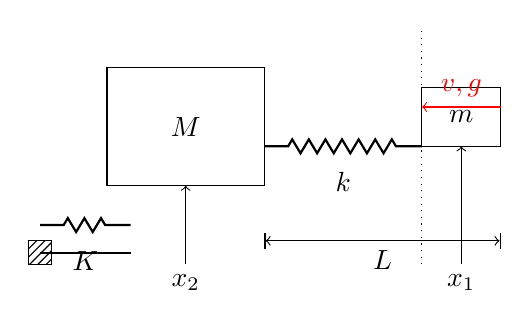
\begin{tikzpicture}[
    spring/.style={
        thick,
        decorate,
        decoration={
            zigzag,
            pre length=0.3cm,
            post length=0.3cm,
            segment length=6
        }
    },
    damper/.style={
        thick,
        dash pattern=on 8pt off 6pt on 2pt off 6pt
    },
    ground/.style={
        fill,
        pattern=north east lines,
        minimum width=0.75cm,
        minimum height=0.3cm
    },
    mass/.style={
        draw,
        outer sep=0pt,
        thick,
        minimum width=2cm,
        minimum height=1.5cm
    },
    label/.style={
        text width=2.5cm,
        align=center,
        minimum height=1.5cm
    }
]

% Ground
\draw[ground] (-1, -1.5) rectangle ++(0.3, 0.3);
\draw[thick] (-0.85, -1.35) -- (0.3, -1.35);

% Spring between ground and mass M
\draw[spring] (-0.85, -1) -- (0.3, -1) node[midway, below=0.2cm] {$K$};

% Mass M
\draw (0, -0.5) rectangle (2, 1) node[midway] {$M$};

% Spring between mass M and mass m
\draw[spring] (2, 0) -- (4, 0) node[midway, below=0.2cm] {$k$};

% Dotted line (reference for mass m)
\draw[dotted] (4, -1.5) -- (4, 1.5);

% Mass m
\draw (4, 0) rectangle (5, 0.75) node[midway] {$m$};

% Labels for displacements
\draw[<-] (1, -0.5) -- (1, -1.5) node[below] {$x_2$};
\draw[<-] (4.5, 0) -- (4.5, -1.5) node[below] {$x_1$};

% Label for length L
\draw[|<->|] (2, -1.2) -- (5, -1.2) node[midway, below] {$L$};

% Velocity and gravity direction
\draw[->, red] (5, 0.5) -- (4, 0.5) node[midway, above] {$v, g$};

\end{tikzpicture}

\end{document}